\chapter{定义和背景}
\label{cha:chap02}

本章主要对于本文的基础算法和涉及到的GPU/CUDA加速技术进行了介绍。首先介绍Shapelet算法的相关定义和通用算法,并对通用算法时间复杂度进行了分析。然后对于不同的相似度度量方法进行了分析和比较,并对部分相似度/距离度量之间关系进行了介绍。最后,详细介绍了GPU/CUDA并行原理以及本文并行工作使用到的CUDA优化技术。

%本章主要对Shapelet及相关工作进行介绍。首先对于Shapelet相关定义及计算过程进行介绍;然后对于不同的相似度度量方法进行了分析和比较;最后对Shapelet算法及面临的问题进行分析并且对Shapelet的已有优化工作进行了分类和比较。

\section{Shapelet相关定义}
\label{cha:chap02:def}
本章节介绍Shapelet的相关定义\cite{ye2009time},这些定义是理解Shapelet发现过程的前提,后文主体部分都是依照本章节进行展开的。

\begin{definition}
	数据集的表示:对于一个时间序列数据集$D$,和其他数据集一样,都是由输入(时间序列)与输出(类标)组成,数据集通常表示为公式~\ref{equ:chap2:Dataset}形式。其中$T_j$是一个时间序列,$y_j$是其类标,其中$y_j\in{A,B}$,这里及后文中$N$表示时间序列个数,即数据集大小。
	\begin{equation}
	\label{equ:chap2:Dataset}
	D = \left\lbrace (T_1,y_1),(T_2,y_2),\cdots (T_N,y_N)\right\rbrace 
	\end{equation}
\end{definition}


\begin{definition}
	时间序列$T_j=t_1,\cdots,t_L$是由$L$个实数组成的有序集合。$t_1,\cdots,t_L$是按时间顺序排列并且具有相同的时间间隔。时间序列$T_j$上的元素$t_p$可以通过$T_{j,p}$来表示。时间序列$T_j$的长度可以用$|T_j|$表示,也可以通过$L$来表示。后文提到的$L$都是数据集中时间序列的长度,而且本文中提到的时间序列都是等长的,长度为$L$。
\end{definition}

\begin{definition}
\label{def:chap02:Subsequence}
	子序列($Subsequence,S$),对于长度为$L$的时间序列$T_j$,对于任何一个子序列可以由两个参数( 起始位置$s$和子序列长度$len$)确定唯一的子序列$T_{j,s}^{len}(s.t.\quad s+len <= L)$。对于任意一个子序列$S$的长度可以通过$|S|$来表示,但不能通过$L$表示。
	
	时间序列$T_j$的子序列集合可以通过$Subset(T_j)$表示,$Subset(T_j)$集合大小为$\frac{L(L+1)}{2}$(这里不包括长度为0的时间序列)。数据$D$的所有子序列集合可以用$SubSet(D)$表示,数据集$D$有$N$个长度为$L$的时间序列,则$SubSet(D)$的集合大小为$\frac{NL(L+1)}{2}$。因为每一个子序列都是Shapelet的候选序列,因此我们把子序列由称为候选序列,$D$对应的子序列集合$SubSet(D)$又称为候选序列集(合)。
\end{definition}

\begin{definition}
	\label{def:chap2:Dist}
	时间(子)序列$A,B$之间的距离$Dist(A,B)$,用于表示具有相同长度的时间(子)序列$A$和时间(子)序列$B$的相似度。
	
	原始Shapelet算法使用欧式距离(Euclidean distance)作为子序列相似度度量,但是作为距离,只要满足对称性、非负性、三角不等式形式的,就可以满足$Dist(A,B)$的要求,这里$Dist(A,B)$可以扩展到其他广义距离,包括曼哈顿距离,欧氏距离,$DTW$距离等。
\end{definition}

\begin{definition}
\label{def:chap2:SubDist}
	候选序列$S$到时间序列$T_j$之间的距离(必须满足$|S|<=|T_j|$),是$T_j$序列中所有长度为$|S|$的子序列与$S$距离$Dist(T_{j,p}^{|S|},S),p=1\to L-|S|+1$的最小值,如公式~\ref{equ:chap2:SubDist}。
	\begin{equation}\label{equ:chap2:SubDist}
		SubDist(S,T_j) = \min\limits_{p=1\to L-|S|+1} (Dist(S,T_{j,p}^{|S|}))
	\end{equation}
	候选序列$S$和数据集$D$的所有时间序列$T_j,j=1,2,\cdots,N$计算距离,可以获得一个$SubDist(S,T_j)$的向量,记作$dist$,如公式~\ref{equ:chap2:SubDistlist}。
	\begin{equation}
	\label{equ:chap2:SubDistlist}
	dist=\left\lbrace SubDist(S,T_1),SubDist(S,T_2),\cdots,SubDist(S,T_N)\right\rbrace
	\end{equation}
	将$dist$中的元素和类标一一对应起来组成的“距离-类标对”的向量,记作$\mathcal{F}$,如公式~\ref{equ:chap2:SubDistSet},其中有$\mathcal{F}_{j,1}=SubDist(S,T_j)$,$\mathcal{F}_{j,2}=y_j$。
	\begin{equation}
	\label{equ:chap2:SubDistSet}
	\mathcal{F} = \left\lbrace (SubDist(S,T_1),y_1),(SubDist(S,T_2),y_2),\cdots,(SubDist(S,T_N),y_N) \right\rbrace 
	\end{equation}
\end{definition}

\begin{definition}
	\label{def:chap02:infogain}
	信息增益,根据特征$A$将训练数据集$D$划分为$M$个子集$D_1,D_2,\cdots,D_M$,特征$A$对于数据集$D$的信息增益$g(D,A)$是数据集D的信息熵$H(D)$和在$A$给定条件下经验条件熵$H(D|A)$之差,即公式~\ref{equ:chap02:Infogain}。$A$特征对应的信息增益越大,则说明特征$A$的分类能力越强,Shapelet使用信息增益作为候选序列筛选的标准。
	\begin{equation}
	\label{equ:chap02:Infogain}
	g(D,A) = H(D) - H(D|A) = H(D) - \sum_{i=1}^{M}\frac{|D_i|}{|D|}H(D_i|A)
	\end{equation}
	候选序列$S$与数据集$D$中每一个时间序列$T_j,j=1,2,\cdots,N$的距离$SubDist(S,T_j)$,其中$SubDist(S,T_j)$的所有取值分布在$(0,\infty)$区间,如图~\ref{fig:SubDist}。候选序列$S$和分割点$d_{th}$共同作为特征$(S,d_{th})$将数据集$D$分为$D_1 = \left\lbrace T_j,SubDist(S,T_j)<d_{th},j=1\to N\right\rbrace $和$D_2 = \left\lbrace T_j,SubDist(S,T_j) \geq d_{th},j=1\to  N\right\rbrace$两部分。特征$(S,d_{th})$相对数据集的信息增益为数据集$D$的信息熵减去子集$D_1$和子集$D_2$的信息熵的权重和,如公式~\ref{equ:chap2:Infogain2}
	\begin{equation}
	\label{equ:chap2:Infogain2}
	g(D,(S,d_{th})) =H(D)-H(D|(S,d_{th})) = H(D)-(\frac{|D_1|}{|D|}H(D_1)+\frac{|D_2|}{|D|}H(D_2))
	\end{equation}	
\end{definition}

\begin{figure}[H] % use float package if you want it here
\centering
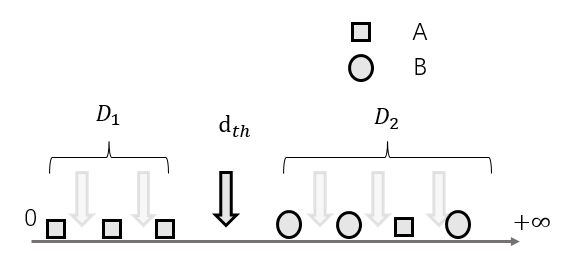
\includegraphics{SubDistDistribution.png}
\caption{$SubDist(S,T_j),T_j\in D$在$(0,\infty)$的分布}
\label{fig:SubDist}
\end{figure}

\begin{definition}
	\label{def:optimalsplitpoint}
	最佳分割点:在候选序列$S$下,有多个分割点$d_{th}$,如图~\ref{fig:SubDist},在这些分割点中,存在一个阈值$d_{osp(S)}$(或者是一段区间),满足$g(D,(S,d_{osp(S)})) \geq g(D,(S,d_{th})),\forall d_{th}\in \mathbb{R}_{+}$,则将$d_{osp(S)}$记为候选序列$S$对应的最佳分割点,而特征$(S,d_{dsp(S)})$在是$S$对应的最佳分割特征。
\end{definition}

数据集$D$中有$O(NL^2)$个候选序列,即有$O(NL^2)$个特征组合$(S,d_{osp(S)})$,需要选取分类能力最高的特征组合,分类能力最高特征组合中的候选序列即为Shapelet,如定义~\ref{def:choose}。

\begin{definition}
	\label{def:choose}
	数据集$D$中的Shapelet,使用$Shapelet(D)$表示。对于给定数据集,存在一个子序列$Shapelet(D)$,使$g(D,(Shapelet(D),d_{osp(Shapelet(D))})) \geq g(D,(S,d_{osp(S)})),\forall S\in SubSet(D)$。$(Shapelet(D),d_{osp(Shapelet(D))})$特征将作为Shapelet算法那最终的分类器。
\end{definition}

\begin{definition}
	\label{def:chap03:Threephases}
	Shapelet计算过程三阶段:本文将Shapelet计算过程分为三个阶段,分别为距离计算阶段、最佳分割点计算阶段、候选序列筛选阶段。其中距离计算阶段是指从候选序列$S$和数据集$D$到$S$相对数据集$D$所有时间序列计算距离获取距离-类标对的集合$\mathcal{F}$的过程,即计算$\mathcal{F}$的过程;最佳分割点计算阶段是指从$\mathcal{F}$到对应的最佳分割点$d_{osp(S)}$以及对应的信息增益的过程,相当于定义~\ref{def:optimalsplitpoint}过程;候选序列筛选阶段是指从多个候选序列根据信息增益选出Shapelet的过程,相当于定义~\ref{def:choose}过程。章节~\ref{cha:chap03:Problemsencountered:BigDataSet}解释了为什么从中间结果$\mathcal{F}$处分成两个阶段,章节~\ref{cha:chap03:modelduty}解释了为了要从最佳分割点处分为两个阶段。
\end{definition}

从以上定义来看,时间序列可以分类的前提是,数据集中的一类(比如$A$类)存在一种模式(波形),这种模式和$A$类时间序列($T_j,y_i\in A$)表现出较小的距离,和另一类$B$类时间序列($T_j,y_i\in B$)表现出较大的距离。而Shapelet算法那就是负责寻找能够区分这两类时间序列的模式以及对应的距离阈值的算法。%Shapelet对于所有的候选序列$(S,d_{osp(S)})$按照对于$D$的信息增益进行评价,选出信息增益最大的候选序列和对应的距离阈值$(Shapelet(D),d_{osp(Shapelet(D))})$。

\section{通用算法分析}
\label{cha:chap02:generalalganalysis}
\begin{algorithm}
	\caption{Shapelet原始算法}
	\label{alg:origin}
	\begin{algorithmic}[1]
		\Function{ShapeletNaiveAlg}{$D$}
		%\State $CENTER \gets (w+1)/2$;
			\State $lastS \gets \phi, lastinfogain \gets 0, lastdosp \gets 0, leftisAorB\gets A$ 
			\ForAll{$S \in SubSet(D)$} \label{Code:Set}
				\State $\mathcal{F} = \left\lbrace (...,SubDist(S,T_j),y_j),...\right\rbrace,j = 1,2,\cdots,N$ \label{Code:calcSubDist}
				\State 计算$g(D,(S,d_{osp(S)}))$ \label{Code:infogain}
				\If{$g(D,(S,d_{osp(S)})) > lastinfogain$}
					\State 更新$lastinfogain$,$lastS$,$lastdospd_{osp(S)}$,$leftisAorB$
				\EndIf
			\EndFor
			\State \Return $lastinfogain,lastS,lastdops,leftisAorB$
		\EndFunction
	\end{algorithmic}
\end{algorithm}

如算法~\ref{alg:origin}为Shapelet发现的通用算法,是所有子序列中发现具有最佳分类能力的子序列的过程。其中:

$line$~\ref{Code:calcSubDist}是对于计算一个候选序列$S$相对于数据集$D$中每个时间序列$T_j$的过程,时间复杂度为$O(NL^2)$;

$line$~\ref{Code:infogain}是寻找一个阈值$d_{osp(S)}$与候选序列$S$配合满足$g(D,(S,d_{osp(S)})) \geq g(D,(S,d_{th})),\forall d_{th}\in \mathbb{R}_{+}$,时间复杂度为$O(N\log(N))$。

$line$~\ref{Code:Set}:$SubSet(D)$集合大小为$O(NL^2)$,因此$line$~\ref{Code:Set}处循环为$O(NL^2)$次;循环内部时间复杂度为$O(NL^2)$。

%对于数据集$D$中所有候选序列$SubSet(D)$都经过$line$~\ref{Code:calcSubDist}-\ref{Code:infogain}两步的评估过程,$SubSet(D)$集合大小为$O(NL^2)$。
因此Shapelet通用算法的时间复杂度为$O(N^2L^4)$,这个时间复杂度非常高,特别$N,L$比较大的情况,严重地影响执行时间。

\section{相似度/距离测度方法}
\label{cha:chap02:Distance}

章节~\ref{cha:chap02:def}描述的相似度/距离计算都是基于两个时间(子)序列$A,B$的相似性度量$Dist(A,B)$进行的,本章节就$Dist(A,B)$展开介绍。时间序列相似性/距离是许多计算系统的核心,同时也是时间序列聚类和分类的最重要的组成部分之一~\cite{patidar2012analysis}。正是由于相似度/距离度量的重要性,多种相似度/距离度量的方法先后被提出。在本章节中,我们对于几个具有代表性的时间序列相似度/距离度量及其所属类别进行评估,相似度/距离计算可以简单分为\cite{ding2008querying}:锁步距离测量(欧氏距离)、基于特征测量(傅里叶系数)、基于模型测量(自回归)、弹性测量(动态时间规整、实数序列的编辑距离)。

在上述多种相似性计算当中,基于特征测量和基于模型测量都没有直接利用时间序列之间的距离而是使用时间序列提取的特征进行计算相似性的,和Shapelet算法的滑动窗口距离取最小值的方法不符,因此对于这两种距离不予考虑。

对于两个时间序列$A=\left\lbrace a_1,a_2,\cdots,a_M\right\rbrace$和$B=\left\lbrace b_1,b_2,\cdots,b_M\right\rbrace$,本章主要讨论欧氏距离、实数序列的编辑距离、动态时间规整距离进行介绍并比较。

\subsection{欧氏距离}
欧氏距离是使用最普遍的距离测度方法,是度量$M$维空间上的两个点的直线距离,使用$Dist(A,B)$或者$Euclid(A,B)$表示。将欧氏距离应用在时间(子)序列上,要求两个时间序列$A,B$的长度相等$|A|=|B|$。在实际使用中经常将欧式距离的定义会进行扩展,使用两个长度相等时间序列$A,B$的差的$L_n$范数作为欧氏距离~\cite{serra2014empirical},如公式~\ref{equ:chap2:DistEuclid}。有时候,为了便于计算,经常使用$\sum_{i=1}^{M}(A_i-B_i)^n$记做欧氏距离,其中$n=1$,为曼哈顿距离,$n=2$,为狭义欧氏距离,$n$一般会作为一个底层距离参数,可以根据情况调节。
\begin{equation}
\label{equ:chap2:DistEuclid}
Euclid(A,B) = (\sum_{i=1}^{M}(A_i-B_i)^n)^{\frac{1}{n}}
\end{equation}

欧氏距离的优点在于计算简单,复杂度低;缺点要求两个时间序列各元素一一对应,不能弹性地计算时间序列之间距离,不能扭曲对应,这也是欧氏距离属于锁步距离的原因。

%对于长度都为$M$的两个时间(子)序列$A$和$B$,两者之间的欧氏距离是两者对应元素平方和的平方根,如~\ref{equ:chap2:DistEuclid}。为了简化计算,经常使用平方和$\sum_{i=1}^{M}(A_i-B_i)^2$表示$Dist(A,B)$。
%
%欧氏距离之所以称为锁步距离,就是需要元素一一对应

\subsection{动态时间规整}
\label{cha:chap02:dtw}


动态时间规整\cite{muller2007dynamic}(Dynamic Time Warping,~DTW)是一种通过将一个时间序列$A$延时间轴进行非线性的延展或者压缩,目的使$A$序列和另一时间序列$B$能够很好地对齐,对齐方式如图~\ref{fig:twoplotdtw}。这种对齐方式是可以通过一种动态规划的算法计算获得,如图~\ref{fig:threeplotdtw},图中从$(0,0)$到$(|A|,|B|)$的路线称为规整路径。

\begin{figure}
	\begin{minipage}{0.48\textwidth}
		\centering
		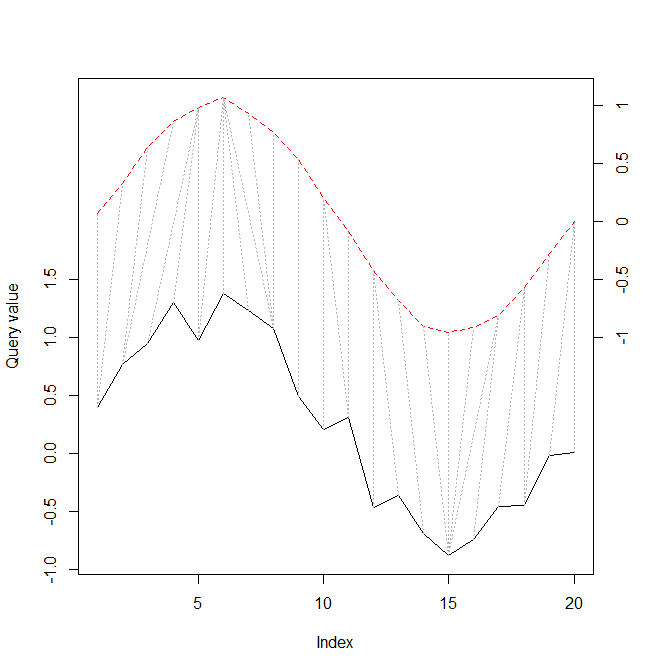
\includegraphics[height=6.2cm]{twoplotdtw.png}
		\caption{时间序列$A,B$对齐方式}
		\label{fig:twoplotdtw}
	\end{minipage}\hfill
	\begin{minipage}{0.48\textwidth}
		\centering
		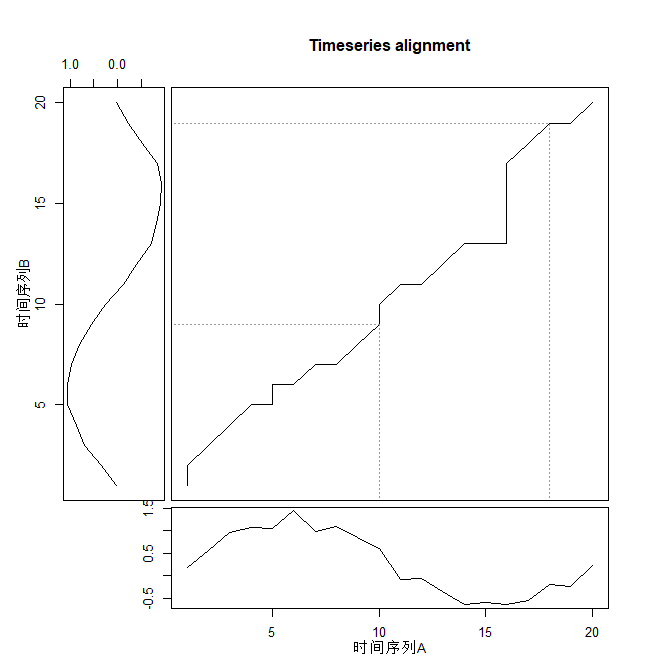
\includegraphics[width=6.2cm]{threeplotdtw.png}
		\caption{时间序列$A,B$规整路径和代价矩阵}
		\label{fig:threeplotdtw}
	\end{minipage}
\end{figure}

$A$和$B$之间的DTW距离用$DTW(A,B)$来表示,$DTW(A,B)$的递归方程如公式~\ref{equ:chap2:costMatrix}~\cite{sart2010accelerating}\footnote{n=1,2}。

\begin{equation}
\label{equ:chap2:costMatrix}
\begin{array}{l}
Dist(A,B) = d(M,M) \\ [0.3cm]
d(i,j) = |a_i-b_j|_n + \min
\begin{cases}
d(i-1,j)\\
d(i,j-1)\\
d(i-1,j-1)
\end{cases}\\[0.2cm]
d(0,0)=0;d(i,0)=\infty;d(0,j)=\infty;i=1,2,\cdots,M;j=1,2,\cdots,M 
\end{array}
\end{equation}


我们要求上面递推公式~\ref{equ:chap2:costMatrix}比较的两个时间序列长度是相等的$|A|=|B|= M$,但其实DTW不要求时间(子)序列长度一致。这里要求$|A|=|B|= M$主要基于两个原因考虑:第一,这样对于任何一个子序列$S$与$T_j$的距离,如果不要求(子)序列长度一致,就必须计算$T_j$所有子序列和$S$的DTW距离,然后在这些距离中取最低值,这样$S$需要和$O(L^2)$个子序列计算距离,使计算的复杂度变高;第二,不能判断哪个时间序列更具相似性,比如有$D,E,F$三个时间序列,其中$|D|<<|E|<|F|$,$DTW(D,E) < DTW(F,E)$,但是这里不能就此认定对于$E$,$D$比$F$更具有相似性。

递归方程~\ref{equ:chap2:costMatrix}计算DTW距离的时间复杂度和空间复杂度都是$O(M^2)$(如果$|A|=|B|=M$),相比于欧氏距离都很大。因为DTW时间空间复杂度高的原因,有人提出了FastDTW\cite{salvador2007toward},通过将规整路径限制在一定区域内来加速计算,限制区域主要包括$Sakoe-Chuba band$(如图~\ref{fig:Sakoe-Chuba-band})和$Itakura band$(如~\ref{fig:Itakura-band})两种方法。这两种限制区域的方式实质上将时间序列扭曲对应限制在一定的范围内。

本文使用到的是Sakoe-Chuba-band限制区域方法,这里需要对它进行介绍。如图~\ref{fig:Sakoe-Chuba-band},Sakoe-Chuba-band限制区域沿反对角线方向向两边延展,而$w$是一个控制限制区域宽度的参数,这里使用$DTW(A,B,w)$表示时间序列$A,B$之间的$w$参数下限制区域DTW距离。$w(w>=0)$作为限制区域的宽度的参数,当$w=0$时,限制区域为反对角线;当$w=M$(与时间序列$A,B$长度相等)时,限制区域为整个代价矩阵区域,这个时候限制区域DTW距离计算退化为于原始的DTW距离。因为$DTW(A,B)$或者$DTW(A,B,w=M)$距离是限制区域$DTW(A,B,w)$距离的特殊形式,后文提到的DTW距离都是指$DTW(A,B,w)$距离,而原始的DTW距离将会用$DTW(A,B,w=M)$来表示。

算法~\ref{alg:fastdtw}是$DTW(A,B,w$距离计算的算法,时间复杂度和空间复杂度都为$O(wM)$。

\begin{figure}
	\begin{minipage}{0.48\textwidth}
		\centering
		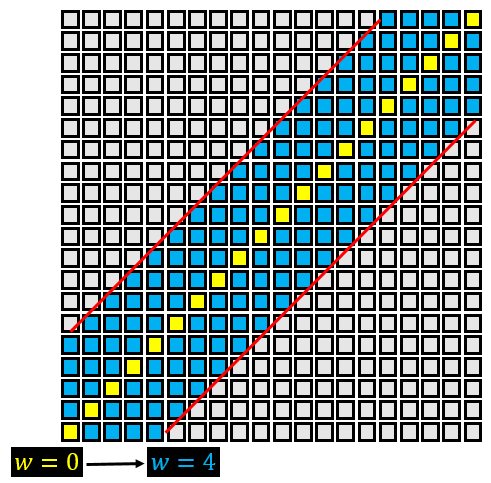
\includegraphics[height=6.2cm]{Sakoe-Chubaband.png}
		\caption{Sakoe-Chuba-band限制区域}
		\label{fig:Sakoe-Chuba-band}
	\end{minipage}\hfill
	\begin{minipage}{0.48\textwidth}
		\centering
		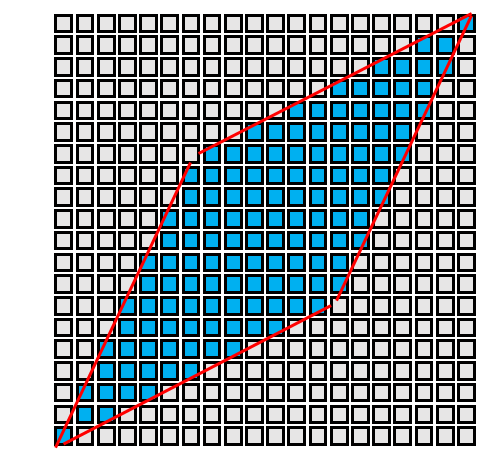
\includegraphics[width=6.3cm]{Itakuraband.png}
		\caption{Itakura-band限制区域}
		\label{fig:Itakura-band}
	\end{minipage}
\end{figure}



\begin{algorithm}
	\caption{DTW距离计算($Sakoe-Chuba-band$限制区域)}
	\label{alg:fastdtw}
	\begin{algorithmic}[1]
		\Function{DTW}{$A,B,w$}  //$|A|=|B|=M$
			\State $D = array(M+1,M+1)$
			\For{$m = 0$ to $M$}
				\If{$m < w$}
					\State $D_{m,0} \gets \infty, D_{0,m} \gets \infty$
				\Else
					\State $D_{m,w+m} \gets \infty, D_{w+m,m} \gets \infty$
				\EndIf
			\EndFor
			
			\For{$m = 1$ to $M$}
				\For{$n = \max(m-w,1)$ to $\min(M,m+w)$}
					\State $D_{m,n} = \min(D_{m-1,n-1},D_{m-1,n},D_{m,n-1}) + d(a_m,b_n)$
				\EndFor
			\EndFor
			\State \Return $D_{M,M}$
		\EndFunction
	\end{algorithmic}
\end{algorithm}

\subsection{实数序列的编辑距离}
实数序列的编辑距离~\cite{chen2005robust}(Edit Distance on Real Sequence,~EDR)可以视为原始编辑距离算法在实数序列领域的扩展,递归方程如公式~\ref{equ:chap2:EDR}。
\begin{equation}
\label{equ:chap2:EDR}
\begin{array}{l}
EDR(A,B) = d(M,M) \\ [0.3cm]
d(i,j) = \begin{cases}
i & \text{if }j=0 \\
j & \text{if } i=0 \\
d(i-1,j-1) & \text{if } \theta(a_i-b_j,\epsilon) \\
\min(d(i,j-1),d(i-1,j-1),d(i-1,j)) + 1 & \text{otherwise} \\
\end{cases}\\[0.2cm]
\end{array}
\end{equation}
EDR要求时间序列长度相等$|A|=|B|$,主要是基于和DTW距离相同的考虑。其中,$\theta$是一个阶跃函数,参数$\epsilon$,$\epsilon\in [0,\infty)$是一个控制两个序列样本$a_i,b_j$是否匹配的阈值参数,在实际的EDR计算中,$\epsilon$作为一个超参数需要提前确定。但是如果将EDR应用到Shapelet中,这样的参数$\epsilon$难以确定,对于某一个数据集适应的$\epsilon$不一定适应于其他数据集。

%,因为在Shapelet发现过程中,存在大量不同长度的候选序列$S_1,S_2,|S_1|\neq |S_2|$和分别和时间序列子序列$T_{j,s}^{|S_1|},T_{j,s}^{|S_2|}$进行距离计算,$EDR(S_1,T_{j,s}^{|S_1|})$和$EDR(S_2,T_{j,s}^{|S_2|})$的计算不能使用相同的$\epsilon$参数来度量距离。


\subsection{欧式距离与动态时间规整比较}
\label{chap02:euclid2Dtw}

%在过去的十年中,已经提出了超过一百种不同的时间序列距离测量方法[12]。 然而越来越多的经验证据表明动态时间翘曲(DTW)(包括欧几里得距离作为一种特殊情况)是跨越广泛领域的最佳测量方法[7]。
%[12]Keogh, E. J. and Kasetty, S. On the Need for Time Series Data Mining Benchmarks: A Survey and Empirical Demonstration. Data Min. Knowl. Discov. 7(4): 349-371 (2003).

如图~\ref{fig:Sakoe-Chuba-band},当$w=0$时,DTW代价矩阵将会退化成代价矩阵的对角线,$D(i,j)$的递推方程也将变为沿对角线递归,如图~\ref{fig:Sakoe-Chuba-band}黄色部分和~\ref{equ:chap2:dtwdeg2euclid1}递归方程,因此,当$w=0$时,时间序列的距离$DTW(A,B,0)$则退化欧式距离。%,如公式~\ref{equ:chap2:dtwdeg2euclid2}

\begin{equation}
\label{equ:chap2:dtwdeg2euclid1}
\begin{array}{l}
d(i,j) = |a_i-b_j|_n + \min
\begin{cases}
d(i-1,j)\\
d(i,j-1)\\
d(i-1,j-1)\\
\end{cases} = |a_i-b_j|_n + d(i-1,j-1)
\\[0.2cm]
d(0,0)=0 \\[0.2cm]
DTW(A,B,0) = d(M,M) = \sum_{i=1}^{M}|a_i-b_i|_n = Euclid(A,B)
\end{array}
\end{equation}

当$w=0$时,在DTW距离计算等价于欧氏距离,但是相比欧式距离会多出$2M$个比较计算过程和$2M$次访存过程。

\section{GPU/CUDA并行原理及相关优化技术}
\label{cha:chap03:gpu-HW-Arch}

GPU/CUDA并行采用单指令多数据(Single Instruction Multiple Data,~SIMD)并行方式的。SIMD并行是将数据元素映射到并行处理线程交由相同的程序处理。本章节首先从GPU硬件架构和CUDA并行原理方面进行介绍并行技术,其中,GPU硬件结构部分介绍GPU的硬件结构组成构成并行的基础,CUDA并行原理部分来说明CUDA如何利用GPU硬件完成并行任务的。然后在GPU/CUDA并行原理的基础上介绍本文用到的CUDA优化技术。GPU加速并行并没有改变算法的时间复杂度,而是在CPU执行时间的基础上除以一个常数,这个常数由两个因素决定,一是GPU结构及流处理器簇个数和每个流处理器簇中流处理器个数,二是与优化技术和算法的结合以及算法本身的实现有关。硬件基础没有办法改变,更多的是依靠算法实现和优化技术,一个高效的优化算法相比一般的优化算法也会有很大的速度区别,比如归约中的$kernel7$相比$kernel1$在$4M$元素下加速倍数为21倍~\cite{harris2007optimizing}。章节~\ref{cha:chap02:coalesced}-章节~\ref{cha:chap02:bankconflict}详细地介绍了本文用到的CUDA优化技术,包括合并存储器访问、隐藏延时、线程束分歧、存储体冲突等

本章节的图~\ref{fig:GPU-HW-Arch}和图~\ref{fig:nvidia-cuda-arch}全部根据文献~\cite{nickolls2009graphics}和文献~\cite{lippert2009nvidia}综合绘制。本章节介绍GPU/CUDA并行和CUDA相关技术都是以英伟达的图形处理器为例介绍的,对于其他加速设备以及并行技术没有覆盖。
\subsection{GPU硬件结构}
\label{cha:chap03:gpu-Hw}
图~\ref{fig:GPU-HW-Arch}介绍了GPU的典型硬件结构,GPU硬件包括了流处理器、流处理器簇、内存(全局、共享、常量等)几个关键部分。下面从这个几个关键部分开始介绍GPU硬件结构。

流处理器(Streaming Processor,SP)是GPU最基本的单元( 计算单元),也是执行一个线程的基本单元,因此SP又称为CUDA核,如图~\ref{fig:GPU-HW-Arch}的SP。

流处理器簇(Stream Multiprocessors,SM)是由一定数量的SP加上指令单元、寄存器、共享内存、L1/L2缓存等组成。从图~\ref{fig:GPU-HW-Arch}可以看出,每个SM是一个SIMD处理单元,由多个SP和一个指令单元组成。而GPU实际上是一个SM的阵列,而SM又是由多个SP组成,GPU进行并行计算的本质就是众多SP共同进行数据计算的过程。以GTX-1080来讲,GPU含有20个SM,每个SM含有128个SP,即在GPU最多可以同时运行$20*128$个线程。
\begin{figure}[H] % use float package if you want it here
	\centering
	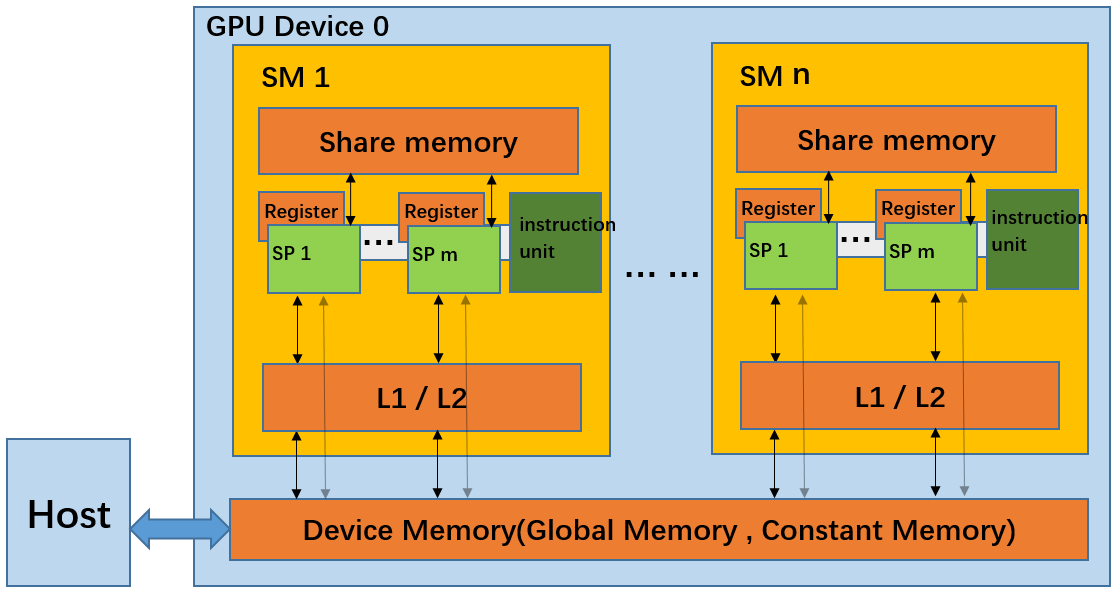
\includegraphics[height=7.2cm]{gpuarch.png}
	\caption{GPU硬件结构}
	\label{fig:GPU-HW-Arch}
\end{figure}

全局内存(Global  memory)是独立于GPU内核的内存,同时也是GPU中空间最大的内存,但访问延时最长,如图~\ref{fig:GPU-HW-Arch}。全局内存有以下特点:对于所有SP可见( 所有SP都可以读写全局内存);可以通过和主存建立主机和GPU之间的数据通信;两个并行任务之间的中间结果必须使用全局内存来处理。

共享内存(Share memory),是存在SM内部可以由SM内部多个线程共享使用的内存,速度是全局内存的几百倍。可以通过共享内存完成线程之间的通信和协作计算。共享内存对于某些特定的线程可见,具体后文会提及。

寄存器(Registers)是GPU中最快的内存,用于存储线程中的临时变量,只在线程内部可见。

本地内存(Local memory)是存储堆栈中无法容纳的所有内容的临时变量,本地内存存储在全局内存中,但对于线程可见。
\begin{table}[htbp]
	\centering
	\begin{minipage}{0.9\textwidth}
		\caption{GPU中各种存储之间的比较}
		\label{tab:memory}
		\begin{tabular}{p{2cm}p{2.1cm}p{3cm}p{2cm}p{2cm}}
			\toprule[1.5pt]
			{\heiti 内存种类} & {\heiti 访存延时} (时钟周期)&{\heiti 内存大小} &{\heiti 可见范围} &{\heiti 周期}\\\midrule[1pt]
			全局内存 & $\sim$400-600 & 8G & 线程网格 & 整个过程 \\
			共享内存 & $\sim$20 & 48K(每个线程块) & 线程块 & 线程 \\
			寄存器 & $\sim$1 & 64K(每个线程块) & 线程块 & 线程 \\
			本地内存 & $\sim$400-600 & 同全局内存 & 线程块 & 线程 \\
			\bottomrule[1.5pt]
		\end{tabular}
	\end{minipage}
\end{table}

常量内存和纹理内存在本文中没有涉及,在这里不做介绍。

表~\ref{tab:memory}对于使用到的内存的性能进行比较,更好地理解各内存在程序中所起的功能。

\subsection{CUDA并行原理}

前面从硬件角度介绍GPU的硬件结构,本章节将从软件角度叙述CUDA如何在GPU的硬件基础进行并行计算的,首先介绍几个CUDA的基本概念。

线程(Thread)是并行程序的基本单元,一个并行程序是由很多线程共同执行,图~\ref{fig:nvidia-cuda-arch}带箭头的曲线表示一个线程。

线程块(Block)由多个线程组成,在一个Block中线程可以进行同步( 需要通过程序控制),也可以通过共享内存进行通信。如图~\ref{fig:nvidia-cuda-arch},每个$Block(x,y)$也是有线程的阵列组成,如$Block(1,1)$。

线程束(Warp),将Block连续线程ID聚合起来的32个线程(比如thread 0-31,32-63)定义为一个Warp,Warp是调度和运行的基本单元,Warp中所有线程并行的执行相同的指令并且是严格同步的,这种同步是由硬件底层完成而不需要通过程序来控制。Block会将连续的32个线程聚合成一个Warp,当一个Block的线程个数不是32个整数倍时,硬件会帮助不足32个线程的部分凑足32个线程形成一个Warp。

%因为SM是一个SIMD处理器,要求所有线程执行相同的指令,如果遇到分支语句,将会将两个分支串行执行。
线程网格(Grid),多个Block构成线程网格,Grid是主机程序调度的接口。如图~\ref{fig:nvidia-cuda-arch}所示,主机调用了两个Grid程序,其中Grid 1是由2*3个Block组成。

\begin{figure}[H] % use float package if you want it here
	\centering
	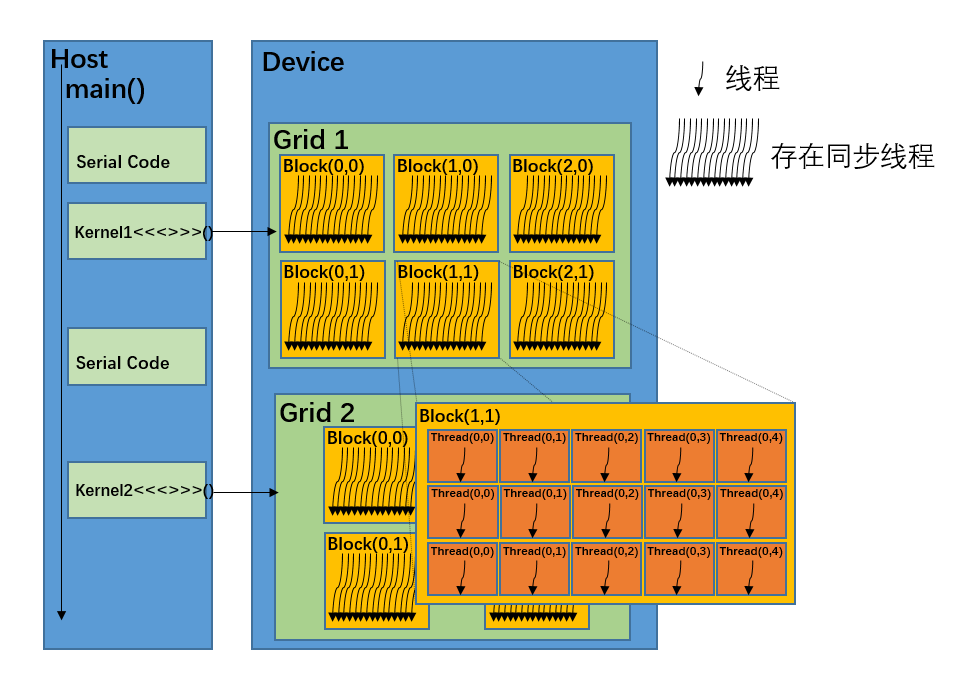
\includegraphics[height=7.5cm]{kernelexcute.png}
	\caption{NVIDIA CUDA架构}
	\label{fig:nvidia-cuda-arch}
\end{figure}

以GTX 1080为例,一个Grid最多可以有$2^{31}-1$个Block,一个Block最多可以有1024个线程,但是在硬件上每个GPU只有20个SM,每个SM只有128个。正常情况下2560个SP是不可能运行这么多线程的。

一个SP只能可以执行一个线程,但是实际上并不是所有的线程能够在同一时刻执行,SM运行线程也是采用了分时复用的思想。连续的32个线程形成一个Warp,一个Block中的1024个线程分成32个Warp。而GTX 1080一个SM有4个Warp调度单元,可以同时容纳4个Warp运行。起初所有Warp都在就绪队列中,首先从就绪对列取出4个Warp在SM上执行;当某个Warp因为读取内存操作或者其他原因而挂起时,Warp调度单元从就绪队列取出一个Warp执行;当正在内存请求的Warp完成内存请求之后,线程束将会进入就绪状态;当线程束执行完任务时进入结束状态;这样不断循环完成一个SM内所有Warp的执行。

多个Warp在4个Warp调度单元通过分时复用的方式进行并行运行,同样道理,一个Grid中大量的Block在20个SM中运行的原理是一致的,都是利用计算资源分时复用的方法。CUDA并行是由成千上万的线程并行完成的,这些线程在软件层面是同时并行的,但是在物理层面最多只有2560个线程在运行,其他都在挂起或者就绪状态。

\subsection{合并存储器访问}
\label{cha:chap02:coalesced}

从表~\ref{tab:memory}可以看出访问全局内存是内存访问耗时最长的环节,但全局内存又是GPU内存最大的部分,当处理大量数据的并行时,不可避免地使用全局内存,这样必然导致大量的全局内存读写操作而产生访存延时,全局内存访问有可能成为性能优化的瓶颈。这里可以通过合并存储器访问~\cite{nvidia2012c}来解决全局内存访问耗时问题。

合并存储器访问(Coalesced Memory Access,~Coalesced),是当特定的访问条件满足时,设备可以将一个Warp内所有线程的全局内存访问操作合并成一个事务。这里特定的条件是一个Warp内线程访问连续的128B空间,而且线程和全局内存地址一一对应( 但不要求严格顺序对齐),如图~\ref{fig:coalesced}~\cite{woolley2013gpu}。这种合并存储器访问模式只需要经过一次L1缓存的过程,大大地提高了全局内存访问速度,由图~\ref{fig:coalesced}红色区域表示。

\begin{figure}[H] % use float package if you want it here
	\centering
	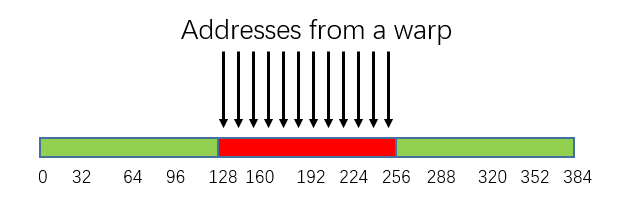
\includegraphics[height=2.5cm]{coaleced.png}
	\caption{合并内存访问(所有线程一个L1缓存行)}
	\label{fig:coalesced}
\end{figure}
合并存储器访问加速全局内存访问可以通过Cache命中观点来解释:当一个Warp的32线程同时读写连续的128B空间,假设某个线程首先读取了128B空间中的某个地址,设备会将这连续的128B空间缓存到L1缓存行中(设备中L1缓存行的大小为128B),其他31个线程再进行读写这个128B地址空间时,可以直接命中到L1缓存行,而Cache的访问时延远小于全局内存,不需要经过内存读写挂起的过程,大大地降低了访问时延。

当一个warp的连续线程访问连续空间但没有按照L1对齐时,会请求两个128B的L1缓存行,如图~\ref{fig:Nocoaleced},会出现两次缓存L1的过程,至少需要经过两个全局内存时延等待。而且这种情况一般会伴随着同一个128B地址被两个warp访问,如果同一个128B地址被两个warp访问,而且这两个warp又不在一个SM中,就会因为考虑数据一致性的问题而导致延时。

\begin{figure}[H] % use float package if you want it here
	\centering
	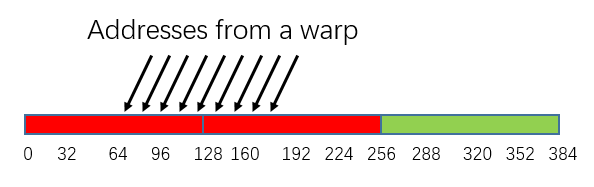
\includegraphics[height=2.5cm]{Nocoaleced.png}
	\caption{非对齐顺序地址访问(使用两个128B)}
	\label{fig:Nocoaleced}
\end{figure}

合并存储器访问大大减少了全局内存访问时延,一般数据量过大的并行计算都是需要全局内存配合合并存储器访问来解决。同时,合并存储器访问、全局内存、共享内存结合使用可以完成很多复杂操作,比如矩阵转置等。

%为了尽量减少全局内存访问延时,减少等待时间,一方面需要增加一个Block内的Warp个数,对于访存时间进行隐藏,另外一方面,使用合并存储器访问减少全局内存访问时延出现的次数。%将一个warp内多个线程计算的结果存储在连续的全局内存地址上,并且保证一个Warp对应能够缓存的128B地址。

\subsection{延时隐藏}

线程不可避免会出现访问各种内存访问而产生的访存延时,为了使访存延时不影响执行速度,可以使用隐藏延时的方法来解决。SM使通过调度Warp来执行线程,可以通过增加Warp的个数来使Warp调度单元尽可能选择已经就绪的Warp,避免选择正在因为延时而挂起的Warp。将通过执行多个Warp来获取较高吞吐量的方法称为隐藏延时。

对于这种性能度量通常通过占用率来评价,占用率通过并行执行的Warp数量除以并发运行的最大可能Warp数量。高占用率意味着Warp调度器有很多Warp可供选择,能够隐藏延时访存等。

在实际优化中,可以对于一个Block中执行的Warp个数进行调节,选择执行时间最短的。另外尽量避免全局内存访存之后出现同步操作,这样容易使访存时间没有办法隐藏。
%如果存在访存等延时尽可能选择较多的warp.
%{\color{red}{按照下面方法计算占有率,这个得做实验}}
%较高的占用率并不总是等同于较高的性能 - 有一点超出额外占用率不会提高性能。 但是,低占用率总是会干扰隐藏内存延迟的能力,从而导致性能下降。在于评价?
%http://docs.nvidia.com/cuda/cuda-c-best-practices-guide/index.html#memory-optimizations    Execution Configuration Optimizations
%尽量增加SM上的线程数量,提高Occupancy(实际并发运行的warp个数/最大可能并发运行的warp个数);
%http://blog.163.com/wujiaxing009@126/blog/static/71988399201709105252458/
%a. 限制条件:# of registers和# of shared memory, 一个SM可以并行处理768 threads
%b. 100%Occupancy: 2 blocks X 384 threads
%3 blocks X 256 threads
%4 blocks X 192 threads
%6 blocks X 128 threads
%8 blocks X 96 threads
%c. 最小存储器延时:Occupancy≥50% and threads/blocks≥128
%(2) Thread block内的线程个数应该是warp size的整数倍,避免在一个warp内有分支语句;
%(3) Grid/Block Size Heuristics;
%a. # of blocks / # of SMs > 1
%每个SM至少有一个thread block可以执行
%b. 更好的选择:# of blocks / # of SMs > 2
%每个SM有多个thread block可以执行
%c. 每个block占用SM一半以下的资源
%d. # of blocks > 100 使得适应将来的结构
%线程指令是在CUDA中顺序执行的,因此,当一个warp暂停或停顿时执行其他warp是隐藏延迟和保持硬件繁忙的唯一方法。 因此,在确定硬件保持繁忙的有效程度时,与多处理器上的活动warp数相关的一些度量标准非常重要。 这个度量是占用率

\subsection{线程束Warp分歧}

因为线程束Warp使GPU调度得基本单元,每个SM又是SIMD处理器(只有一个指令单元,但有多个处理器),因此Warp内的线程只能执行同一条指令。当遇到分支语句时,不同的线程需要执行不同的语句,这和Warp内线程只能执行一个指令互相矛盾。为了解决这个矛盾,分支语句会被序列化,一个Warp中同时只能执行一个分支即部分线程执行,其他分支的线程都处于挂起状态,这样会导致性能的降低,这种现象称为线程束分歧(Warp divergence,Warp分歧)。

为了Warp分歧影响GPU并行效率,尽量避免同一个Warp存在不同的分支路径,如果不能避免Warp分歧的出现,则尽量保证Warp内少数线程执行的分支内容尽可能少,或者提前并行计算。

\subsection{共享内存使用和存储体冲突}
\label{cha:chap02:bankconflict}

前面提到共享内存,相比全局内存拥有更小的时延和更高的带宽,并且线程之间可以通过共享内存进行通信和协作计算,但是使用共享内存有一个前提条件:不能出现存储体冲突。

首先看一下SM中共享内存结构,一个SM上的共享内存实际上是被分为可以同时访问的同等大小的内存块(Bank),因此可以达到共享通信和增加带宽的作用。共享内存中的地址以4bytes为单位依次分配到16个存储体(Bank)中,如图~\ref{fig:bank},$\_\_share\_\_\quad int\quad data[128]$,假设,那么$data[0],data[16],\cdots$属于Bank0,$data[1],data[17],\cdots$属于Bank1,...。

当每个线程(半个Warp)访问不同Bank时,可以快速读写共享内存,如图~\ref{fig:NobankConflict}。但当出现多个线程(半个Warp内)同时访问一个Bank的不同地址时,就会出现存储体冲突(Bank Conflict),这多个线程的访问将被序列化,分先后访问存储体(这部分工作是由硬件完成的),会造成多倍的访问时延,如图~\ref{fig:bankConflict},每个存储体被两个线程访问称为2-way Bank Conflict。但是有一个特殊情况,当一个Warp内的所有线程访问一个存储体中的同一个地址时,共享内存会将这个地址下的数据广播到Warp所有线程中,本文没有涉及,不作详述。

\begin{figure}
	\begin{minipage}{0.3\textwidth}
		\centering
		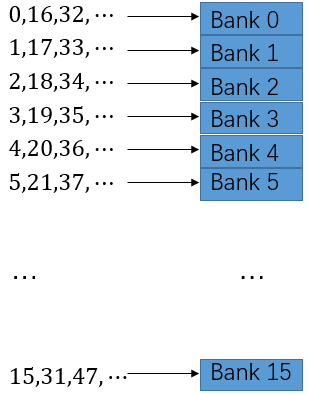
\includegraphics[height=6.2cm]{bank.png}
		\caption{共享内存存储体}
		\label{fig:bank}
	\end{minipage}
	\hfill
	\begin{minipage}{0.30\textwidth}
		\centering
		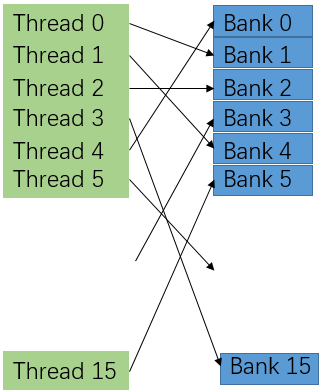
\includegraphics[height=6.2cm]{banknoconflict.png}
		\caption{No bank Conflict}
		\label{fig:NobankConflict}
	\end{minipage}
	\hfill
	\begin{minipage}{0.30\textwidth}
		\centering
		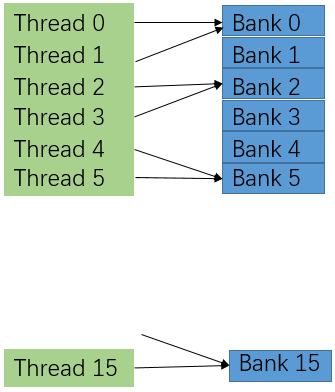
\includegraphics[height=6.2cm]{bankconflict.png}
		\caption{bank Conflict}
		\label{fig:bankConflict}
	\end{minipage}
\end{figure}

Bank Conflict经常出现在多个线程访问不连续的共享内存的情况下,当线程之间访问的共享内存间隔(Stride,4Bytes计为一个间隔)为固定的某个数比如2时,则每两个线程(thread0和thread9,thread1和thread10...)就会访问同一个存储体Bank,这样就会产生存储体冲突(Bank Conflict)。为了避免出现存储体冲突(Bank Conflict)现象,可以通过以下方法避免:

1.最好确保一个Warp的线程访问连续的一块共享内存,线程就能够访问到不同的存储体中;

2.使连续线程访问不连续共享内存地址,可以对其进行调整,比如访问矩阵的列,可以对矩阵先进行转置;

3.使用数据对齐的方式,尽量使用$int,float$占据4Bytes的格式,避免使用$double$等数据格式;

4.当线程不能访问连续的地址,而且访问的地址之间存在一个stride,需要保证stride=1,3,5,7,9...等奇数。


\section{本章小结}
%本章主要对于本文的基础算法和涉及到的GPU/CUDA加速技术进行了介绍。首先介绍Shapelet算法的相关定义和通用算法,并对通用算法时间复杂度进行了分析。然后对于不同的相似度度量方法进行了分析和比较,最后,详细介绍了GPU/CUDA并行原理以及本文并行工作使用到的CUDA优化技术。

本章首先介绍了Shapelet的相关定义和计算过程,为本文展开工作铺垫基础。然后对于Shapelet通用算法进行了描述,并分析了其时间复杂度,指明了Shapelet发现过程耗时的原因。之后对不同的相似度/距离度量方法进行了比较和分析,并对部分相似度/距离度量之间关系进行了介绍。最后对于GPU/CUDA并行原理和后文使用到的CUDA优化技术进行了详细介绍,为后文并行工作的描述打下基础。


